\documentclass[]{article}
\usepackage{lmodern}
\usepackage{amssymb,amsmath}
\usepackage{ifxetex,ifluatex}
\usepackage{fixltx2e} % provides \textsubscript
\ifnum 0\ifxetex 1\fi\ifluatex 1\fi=0 % if pdftex
  \usepackage[T1]{fontenc}
  \usepackage[utf8]{inputenc}
\else % if luatex or xelatex
  \ifxetex
    \usepackage{mathspec}
  \else
    \usepackage{fontspec}
  \fi
  \defaultfontfeatures{Ligatures=TeX,Scale=MatchLowercase}
\fi
% use upquote if available, for straight quotes in verbatim environments
\IfFileExists{upquote.sty}{\usepackage{upquote}}{}
% use microtype if available
\IfFileExists{microtype.sty}{%
\usepackage{microtype}
\UseMicrotypeSet[protrusion]{basicmath} % disable protrusion for tt fonts
}{}
\usepackage[margin=1in]{geometry}
\usepackage{hyperref}
\hypersetup{unicode=true,
            pdftitle={Notice du démonstrateur},
            pdfborder={0 0 0},
            breaklinks=true}
\urlstyle{same}  % don't use monospace font for urls
\usepackage{graphicx,grffile}
\makeatletter
\def\maxwidth{\ifdim\Gin@nat@width>\linewidth\linewidth\else\Gin@nat@width\fi}
\def\maxheight{\ifdim\Gin@nat@height>\textheight\textheight\else\Gin@nat@height\fi}
\makeatother
% Scale images if necessary, so that they will not overflow the page
% margins by default, and it is still possible to overwrite the defaults
% using explicit options in \includegraphics[width, height, ...]{}
\setkeys{Gin}{width=\maxwidth,height=\maxheight,keepaspectratio}
\IfFileExists{parskip.sty}{%
\usepackage{parskip}
}{% else
\setlength{\parindent}{0pt}
\setlength{\parskip}{6pt plus 2pt minus 1pt}
}
\setlength{\emergencystretch}{3em}  % prevent overfull lines
\providecommand{\tightlist}{%
  \setlength{\itemsep}{0pt}\setlength{\parskip}{0pt}}
\setcounter{secnumdepth}{0}
% Redefines (sub)paragraphs to behave more like sections
\ifx\paragraph\undefined\else
\let\oldparagraph\paragraph
\renewcommand{\paragraph}[1]{\oldparagraph{#1}\mbox{}}
\fi
\ifx\subparagraph\undefined\else
\let\oldsubparagraph\subparagraph
\renewcommand{\subparagraph}[1]{\oldsubparagraph{#1}\mbox{}}
\fi

%%% Use protect on footnotes to avoid problems with footnotes in titles
\let\rmarkdownfootnote\footnote%
\def\footnote{\protect\rmarkdownfootnote}

%%% Change title format to be more compact
\usepackage{titling}

% Create subtitle command for use in maketitle
\providecommand{\subtitle}[1]{
  \posttitle{
    \begin{center}\large#1\end{center}
    }
}

\setlength{\droptitle}{-2em}

  \title{Notice du démonstrateur}
    \pretitle{\vspace{\droptitle}\centering\huge}
  \posttitle{\par}
    \author{}
    \preauthor{}\postauthor{}
    \date{}
    \predate{}\postdate{}
  

\begin{document}
\maketitle

Ce démonstrateur comporte 6 onglets. Pour chacuns d'entre eux, vous
trouverez les explications ci-dessous.

\hypertarget{comment-utiliser-ce-duxe9monstrateur}{%
\subsection{Comment utiliser ce
démonstrateur}\label{comment-utiliser-ce-duxe9monstrateur}}

Page d'accueil. Cliquez sur le bouton de téléchargement afin de pouvoir
lire sur cette notice.

\hypertarget{quest-ce-quun-svm}{%
\subsection{Qu'est ce qu'un SVM?}\label{quest-ce-quun-svm}}

Si vous n'avez pas de notion en terme de machine learning, nous vous
expliquons ici brièvement la méthode des machines à vecteur de support
(SVM) . Cette courte introduction est inspiré du cours de Christophe
Hurlin, que vous pouvez retrouver en intégralité en cliquant sur le lien
ci-dessous:\\
\url{https://sites.google.com/view/christophe-hurlin/teaching-resources/support-vector-machine}.

\hypertarget{pruxe9sentation-de-nos-donnuxe9es}{%
\subsection{Présentation de nos
données}\label{pruxe9sentation-de-nos-donnuxe9es}}

Vous trouverez ici toutes les informations sur les données que nous
avons utilisées pour construire ce démonstrateur. Vous pouvez retrouver
la base de données sur le site de kaggle, en cliquant sur le lien ci
dessous:\\
\url{https://www.kaggle.com/mlg-ulb/creditcardfraud}.

De plus, nous vous expliquons les indices de performances que nous
utilisons dans notre analyse.

\hypertarget{intuxe9raction-avec-le-svm}{%
\subsection{Intéraction avec le SVM}\label{intuxe9raction-avec-le-svm}}

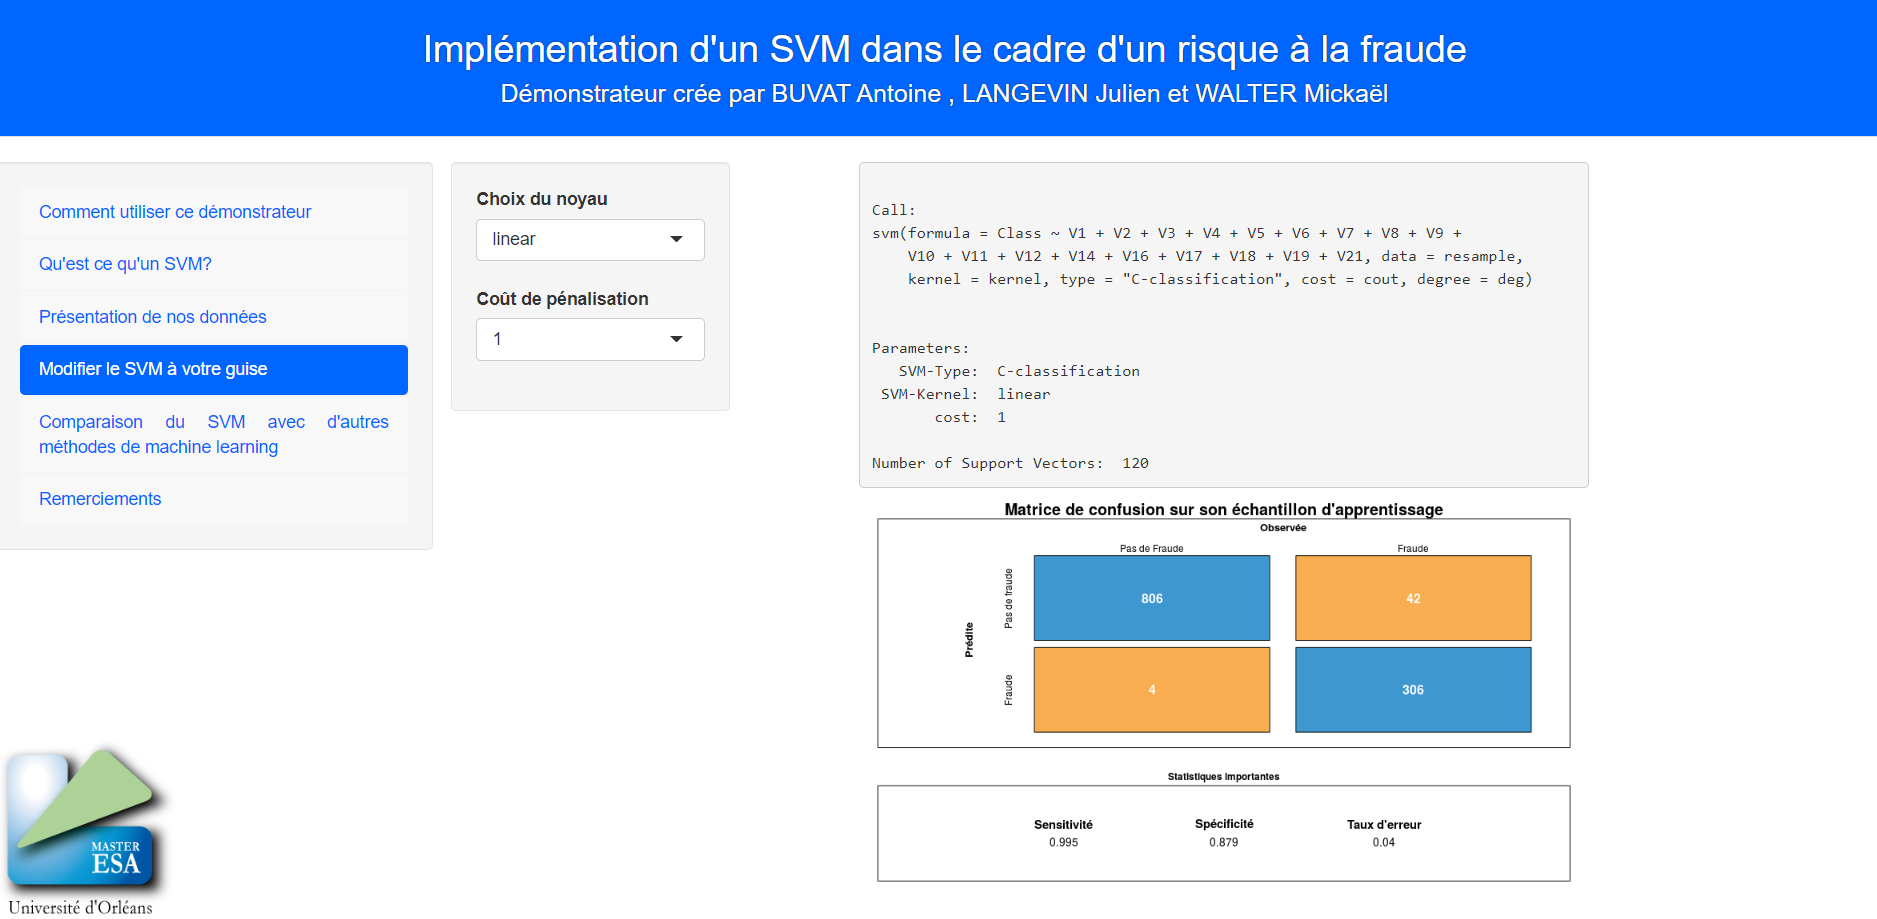
\includegraphics[width=1\linewidth]{C:/Users/mikew/OneDrive/Documents/GitHub/buvat_langevin_walter/www/capture}

Ici, nous montrons les matrices de confusions sur l'échantillon
d'apprentissage et sur l'échantillon test (les observations bien
classées sont en bleu, les autres en oranges), la sensitivité, la
spécificité et le taux d'erreur qui leurs sont associées, ainsi que la
courbe ROC obtenu par la méthode du SVM.

Cette page est intéractive. Ainsi, vous pouvez choisir:\\
- \textbf{La fonction noyau} qui permettra de rendre l'échantillon
linéairement séparable (linéaire, polynomial, radial ou sigmoïde).\\
- \textbf{Le degré du polynôme} que l'on peut fixer à 3, 4 ou 5 que si
nous avons choisi le kernel polynomial.\\
- \textbf{Le coût de pénalisation}, que l'on peut fixer à 1,3,5 ou 10.
Pour rappel, plus ce dernier est important, plus on fait d'erreur, plus
il est grand, plus on risque de faire de l'overfeeting.

\hypertarget{comparaison-du-svm-avec-les-autres-muxe9thdes-de-machines-learning}{%
\subsection{Comparaison du SVM avec les autres méthdes de machines
learning}\label{comparaison-du-svm-avec-les-autres-muxe9thdes-de-machines-learning}}

Cet onglet se décompose en quatre parties distinctes:

\hypertarget{recherche-du-meilleur-svm}{%
\subsubsection{Recherche du meilleur
SVM}\label{recherche-du-meilleur-svm}}

Page d'introduction de l'onglet. On explique brievement la comparaison
des méthodes.

\hypertarget{ruxe9gression-logistique}{%
\subsubsection{Régression logistique}\label{ruxe9gression-logistique}}

On compare les résulats du SVM à ceux de la régression logistique.

\hypertarget{arbre-de-ruxe9gression}{%
\subsubsection{Arbre de régression}\label{arbre-de-ruxe9gression}}

On compare les résultat du SVM à ceux de l'arbre de classification.

\hypertarget{muxe9thode-knn}{%
\subsubsection{Méthode KNN}\label{muxe9thode-knn}}

On compare les résultat du SVM à ceux de la méthode des plus proches
vosins. Dans cette page, vous pourrez modifier le nombre de voisins qui
seront utilisés lors de l'estimation de la méthode KNN (allant de 1 à 20
voisins).

\hypertarget{remerciements}{%
\subsection{Remerciements}\label{remerciements}}

Un dernier onglet où nous vous donnons le lien de notre page Github. Sur
cette page internet, vous trouverez l'ensemble des codes et des
ressources que nous avons utilisé pour la création de ce
démonstrateur.\\
Nous citons aussi les personnes qui nous ont été d'une grande importance
lors de la création de ce projet.


\end{document}
